\subsection{Visualization of the Weights}
We also conducted experiments on the weights of parameters $\boldsymbol{\alpha}_t$ and $\boldsymbol{\beta}_t$ over training steps on the EchoNet-Dynamic dataset, as shown in \cref{fig:wei:echo}. 

These figures show how $\boldsymbol{\alpha}_t$ (controlling memory decay) and $\boldsymbol{\beta}_t$ (balancing old and new information) evolve over training. Their values fluctuate roughly between $-0.06$ and $+0.06$, and they often become more concentrated or exhibit recurring ``hot spots'' as training progresses. Such distributions suggest that the model continually adjusts these gating factors to align with changing task demands, eventually reaching relatively stable (or task-optimal) regions.

%
            \begin{figure}[thpb]
    \centering
        \begin{subfigure}{0.49\linewidth}
		\centering
		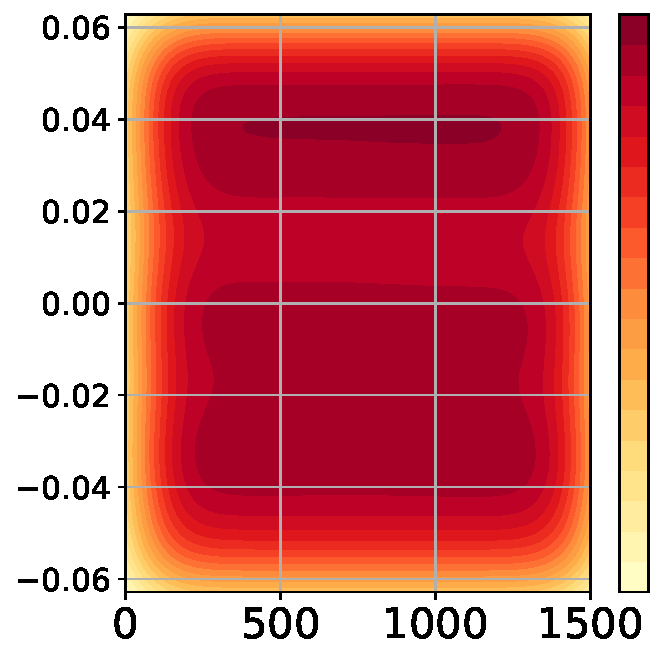
\includegraphics[width=1.0\linewidth]{fig/weight_echo/Para_a.pdf}
		\caption{Distribution of parameter $\boldsymbol{\alpha}_t$. Darker regions indicate higher density.} 
		\label{fig:wei:para_a:echo}
	\end{subfigure}
        %
	\begin{subfigure}{0.49\linewidth}
		\centering
		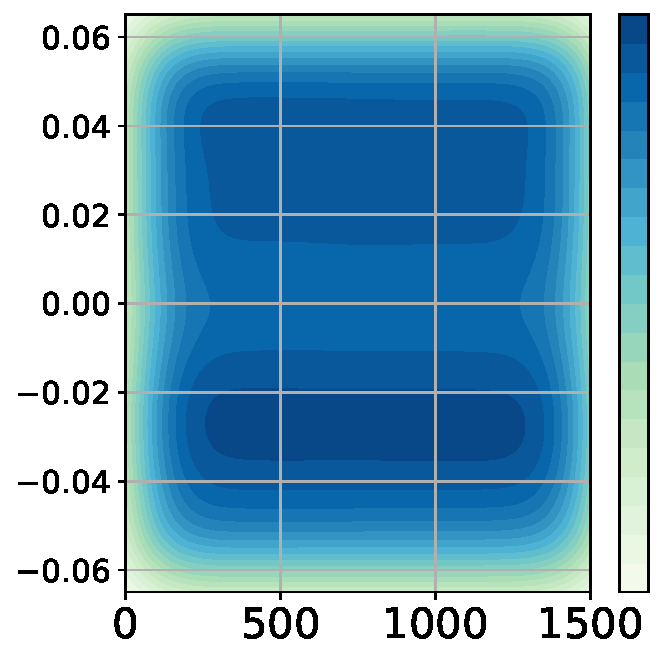
\includegraphics[width=1.0\linewidth]{fig/weight_echo/Para_b.pdf}
		\caption{Distribution of parameter $\boldsymbol{\beta}_t$. Darker regions indicate higher density.} 
		\label{fig:wei:para_b:echo}
	\end{subfigure}
	%\qquad
	\begin{subfigure}{0.49\linewidth}
		\centering
		
\includegraphics[width=1.0\linewidth]{fig/weight_echo/Grad_a_b.pdf}
		\caption{Distribution of gradient $\boldsymbol{\alpha}_t$ and $\boldsymbol{\beta}_t$.}
		\label{fig:wei:Grad:echo}
	\end{subfigure}
        \hspace{0.03mm}
	\begin{subfigure}{0.49\linewidth}
		\centering
		\includegraphics[width=1.0\linewidth]{fig/weight_echo/person_Grad_a_b.pdf}
		\caption{Pearson Correlation of gradient $\boldsymbol{\alpha}_t$ and $\boldsymbol{\beta}_t$. }
		\label{fig:wei:person:echo}
	\end{subfigure}
    \caption{Weights of parameters $\boldsymbol{\alpha}_t$ and $\boldsymbol{\beta}_t$ over training steps on EchoNet-Dynamic.}
    \label{fig:wei:echo}
\end{figure}
%

Although the gradients for these parameters frequently display positive or negative spikes, most gradient values remain within a stable range. This indicates that the network periodically makes significant adjustments to ``forget'' old information or to ``retain'' it when needed. Large gradient magnitudes can pose training challenges, highlighting the importance of proper learning rate settings, gradient clipping, or regularization.

Across different value ranges, the gradients of $\alpha$ and $\beta$ can correlate positively or negatively, forming visually distinct blocks or diagonal patterns. In certain ranges, an increase in $\alpha$ (faster memory decay) may coincide with an increase in $\beta$ (boosting new information), whereas in other ranges $\alpha$ and $\beta$ change in opposite directions. These patterns reflect how the network coordinates the interplay between forgetting past data and incorporating new inputs.

First, $\alpha$ and $\beta$ are learnable rather than fixed, undergoing notable shifts throughout training to accommodate evolving tasks. 
Second, their correlated gradients reveal how the model dynamically manages memory decay and integration to address varying environments or data patterns. 
Third, occasional extreme gradient values suggest training instability when balancing ``forget--retain'' operations, emphasizing the need for methods that mitigate abrupt parameter changes. 
If further experiments show that final values of $\alpha$ and $\beta$ strongly influence performance---for instance, by adopting larger $\alpha$ in scenarios requiring rapid forgetting---it would confirm that this learnable gating mechanism indeed supports the flexible discarding of outdated information.